% $ platex body
% $ dvipdfmx body

\documentclass[a4j]{jarticle}

\title{「西洋音楽の歴史と理論」報告課題}
\author{KR17074 山内 拓弥}
\date{平成29年9月xx日}
\usepackage{colortbl}
\usepackage[dvipdfmx]{graphicx}
%\renewcommand{\thesection}{課題\arabic{section}}
%\renewcommand{\thesubsection}{}

\begin{document}

%\maketitle

\section{中世封建社会の解体}

ヨーロッパ中世の封建社会において、
国王である主君から荘園と呼ばれる領土を与えられた領主は、
その領土の見返りとして軍事的に奉仕する契約を結ぶ。
主君が契約を破れば、臣下である領主も契約を拒否する権利があった。
また、領主は契約の内容以上に主君に尽くす義務は無かった。
このように、中世ヨーロッパの封建制は、
領主の立場が比較的強かった。
この時期、ヨーロッパで最も権力を持っていたのは、ローマ教皇であった。
しかし、1096年から1291年にわたる十字軍の遠征とその失敗により、
ローマ教皇の権威が低下した。
また、十字軍の遠征により、領主が疲弊、没落し、
国王が領主の土地を没収し、国王の権力が高まった。
14世紀頃から貨幣経済がヨーロッパにいきわたり、
余剰生産物の売却などにより農民の地位が向上した。
また、このような社会の変化に対応できずに没落した領主の土地を大商人が購入し、
新しい領主となっていった。
荘園制を基盤とする封建社会は次第に解体し、
貨幣経済と王権を基盤とする社会に変わっていく。

\begin{table}[tb]
 \begin{center}
  \caption{西ヨーロッパ中世とルネサンスの比較}
  \label{tab:comparison}
  \begin{tabular}{|l|l|} \hline
  中世                       & ルネサンス                         \\
  \hline \hline
  教皇が絶大な権力を持つ。   & 教皇の権威が低下、国王が力を持つ。 \\ \hline
  神が中心。                 & 人間が中心。                       \\ \hline
  地球は平坦、天動説。       & 地球は球形、地動説。               \\ \hline
  和音は、神学的理論を優先。 & 和音は、人間の聴覚を優先。         \\
  5度音程が中心。            & 3度、6度のやわらかい響きを多用。   \\ \hline
  \end{tabular}
 \end{center}
\end{table}

\section{ルネサンスの音楽}

\begin{figure}[tb]
 \begin{center}
  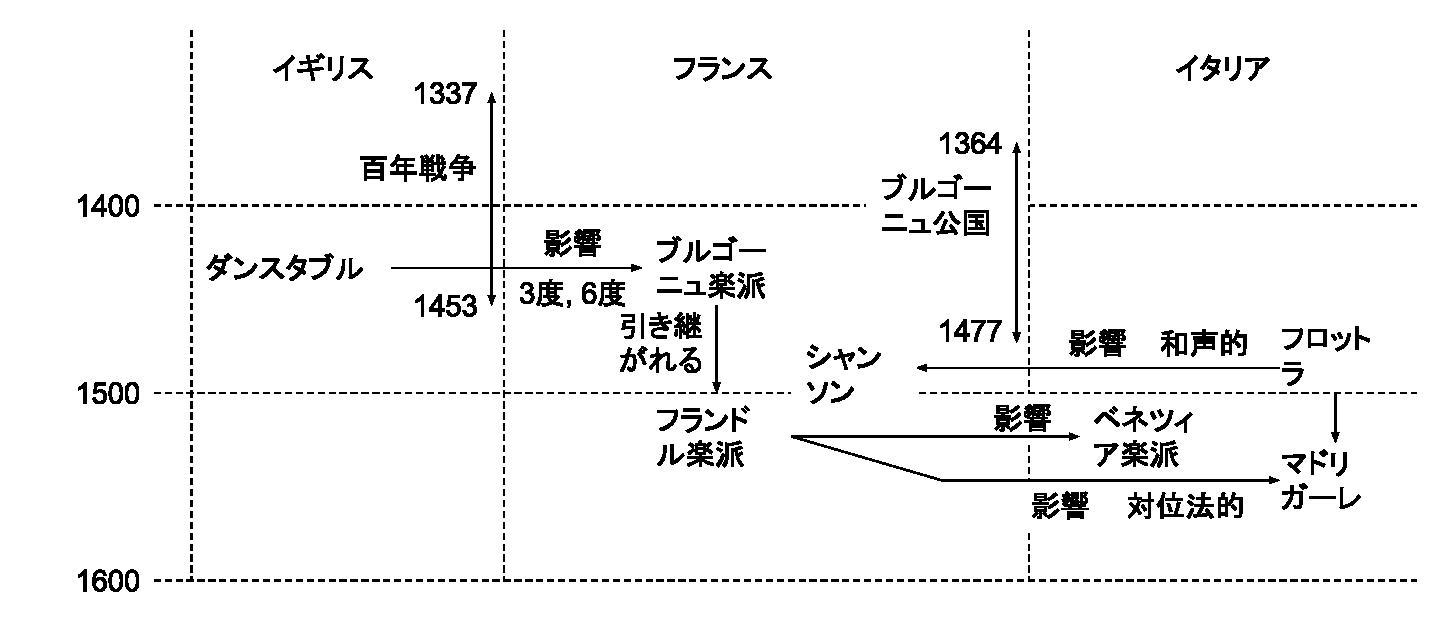
\includegraphics[width=\hsize]{fig/renaissance_summary.eps}
  \caption{ルネサンス音楽概略}
  \label{fig:renaissance_summary}
 \end{center}
\end{figure}

\end{document}
